\section{Svolgimento delle misure}
	La nostra misurazione si compone di due diverse
	fasi: una fase di calibrazione
	dell'apparato ed una fase in cui vengono
	effettuate la misure per determinare $\lambda_{\text{Na}}$.
\subsection{Calibrazione con lampada al cadmio}
	La prima fase consiste nell'azzeramento del dispositivo;
	per fare ciò abbiamo rimosso il prisma ed allineato la
	fenditura di uscita della sorgente,la fessura della slitta
	ed il reticolo a croce del telescopio di osservazione.
	Per effettuare tale allineamento sono state impiegate
	le viti per effettuare spostamenti fini di cui è dotato il piatto
	rotante.

	Abbiamo assunto la lettura del goniometro
	$\alpha_0$ quale zero di riferimento per le successive misure.
	Essendo tale misura basilare per le osservazioni successive
	abbiamo iterato tale misurazione più volte
	ottenendo $\alpha_0 = \angerr{0}{0(1)}$.
	Effettuato questo primo step abbiamo reinserito il
	prisma orientandolo in maniera che formi un angolo
	di circa \ang{60}.

	Si è ruotato il telescopio di osservazione fino ad osservare
	tutte le righe nel visibile emesse dalla nostra sorgente, la lampada al
	cadmio.
	Ruotando ulteriormente il prisma si osserva che le righe si spostano inizialmente
	verso destra (verso angoli minori), per poi cambiare direzione e spostarsi verso
	sinistra (verso angoli maggiori):
	si è bloccato il prisma all'angolo di inversione della direzione di spostamento
	della riga verde (che corrisponderebbe alla condizione di minima deviazione
	per quella riga);
	l'emissione più vicina in lunghezza d'onda a quella che
	intendiamo misurare sarebbe la riga rossa, ma riteniamo che scegliendo una
	riga meno lontana dalle altre righe del cadmio si ottenga una calibrazione migliore.
	Si sono dunque misurate le varie posizioni angolari
	delle righe di emissione della lampada al cadmio.

	\begin{table}[hb]
		\centering
		\begin{tabular}{S[%
			table-figures-decimal = 1,
			table-figures-integer = 3,
			table-figures-uncertainty = 0] r}
			\toprule
			{$\lambda $ [\si{\nm}]} & $ \alpha - \alpha_0 $ \\
			\midrule
			643.8 & \angerr{47}{49 (2)} \\
			508.6 & \angerr{49}{4 (2)} \\
			480.0 & \angerr{49}{31 (2)} \\
			467.8 & \angerr{49}{44 (2)} \\
			441.6 & \angerr{50}{18 (2)} \\
			\bottomrule
		\end{tabular}
		\caption{Posizione angolari delle righe di emissione.}
		\label{tab:disper_angolare}
	\end{table}

	Nel grafico in \fig{fit_a} si è riportata la posizione angolare contro l'inverso della
	lunghezza d'onda per poi verificarne l'andamento lineare con un fit a
	due parametri $\alpha = m \inv{\lambda} + q $.

	\begin{figure} [h]
		\centering
		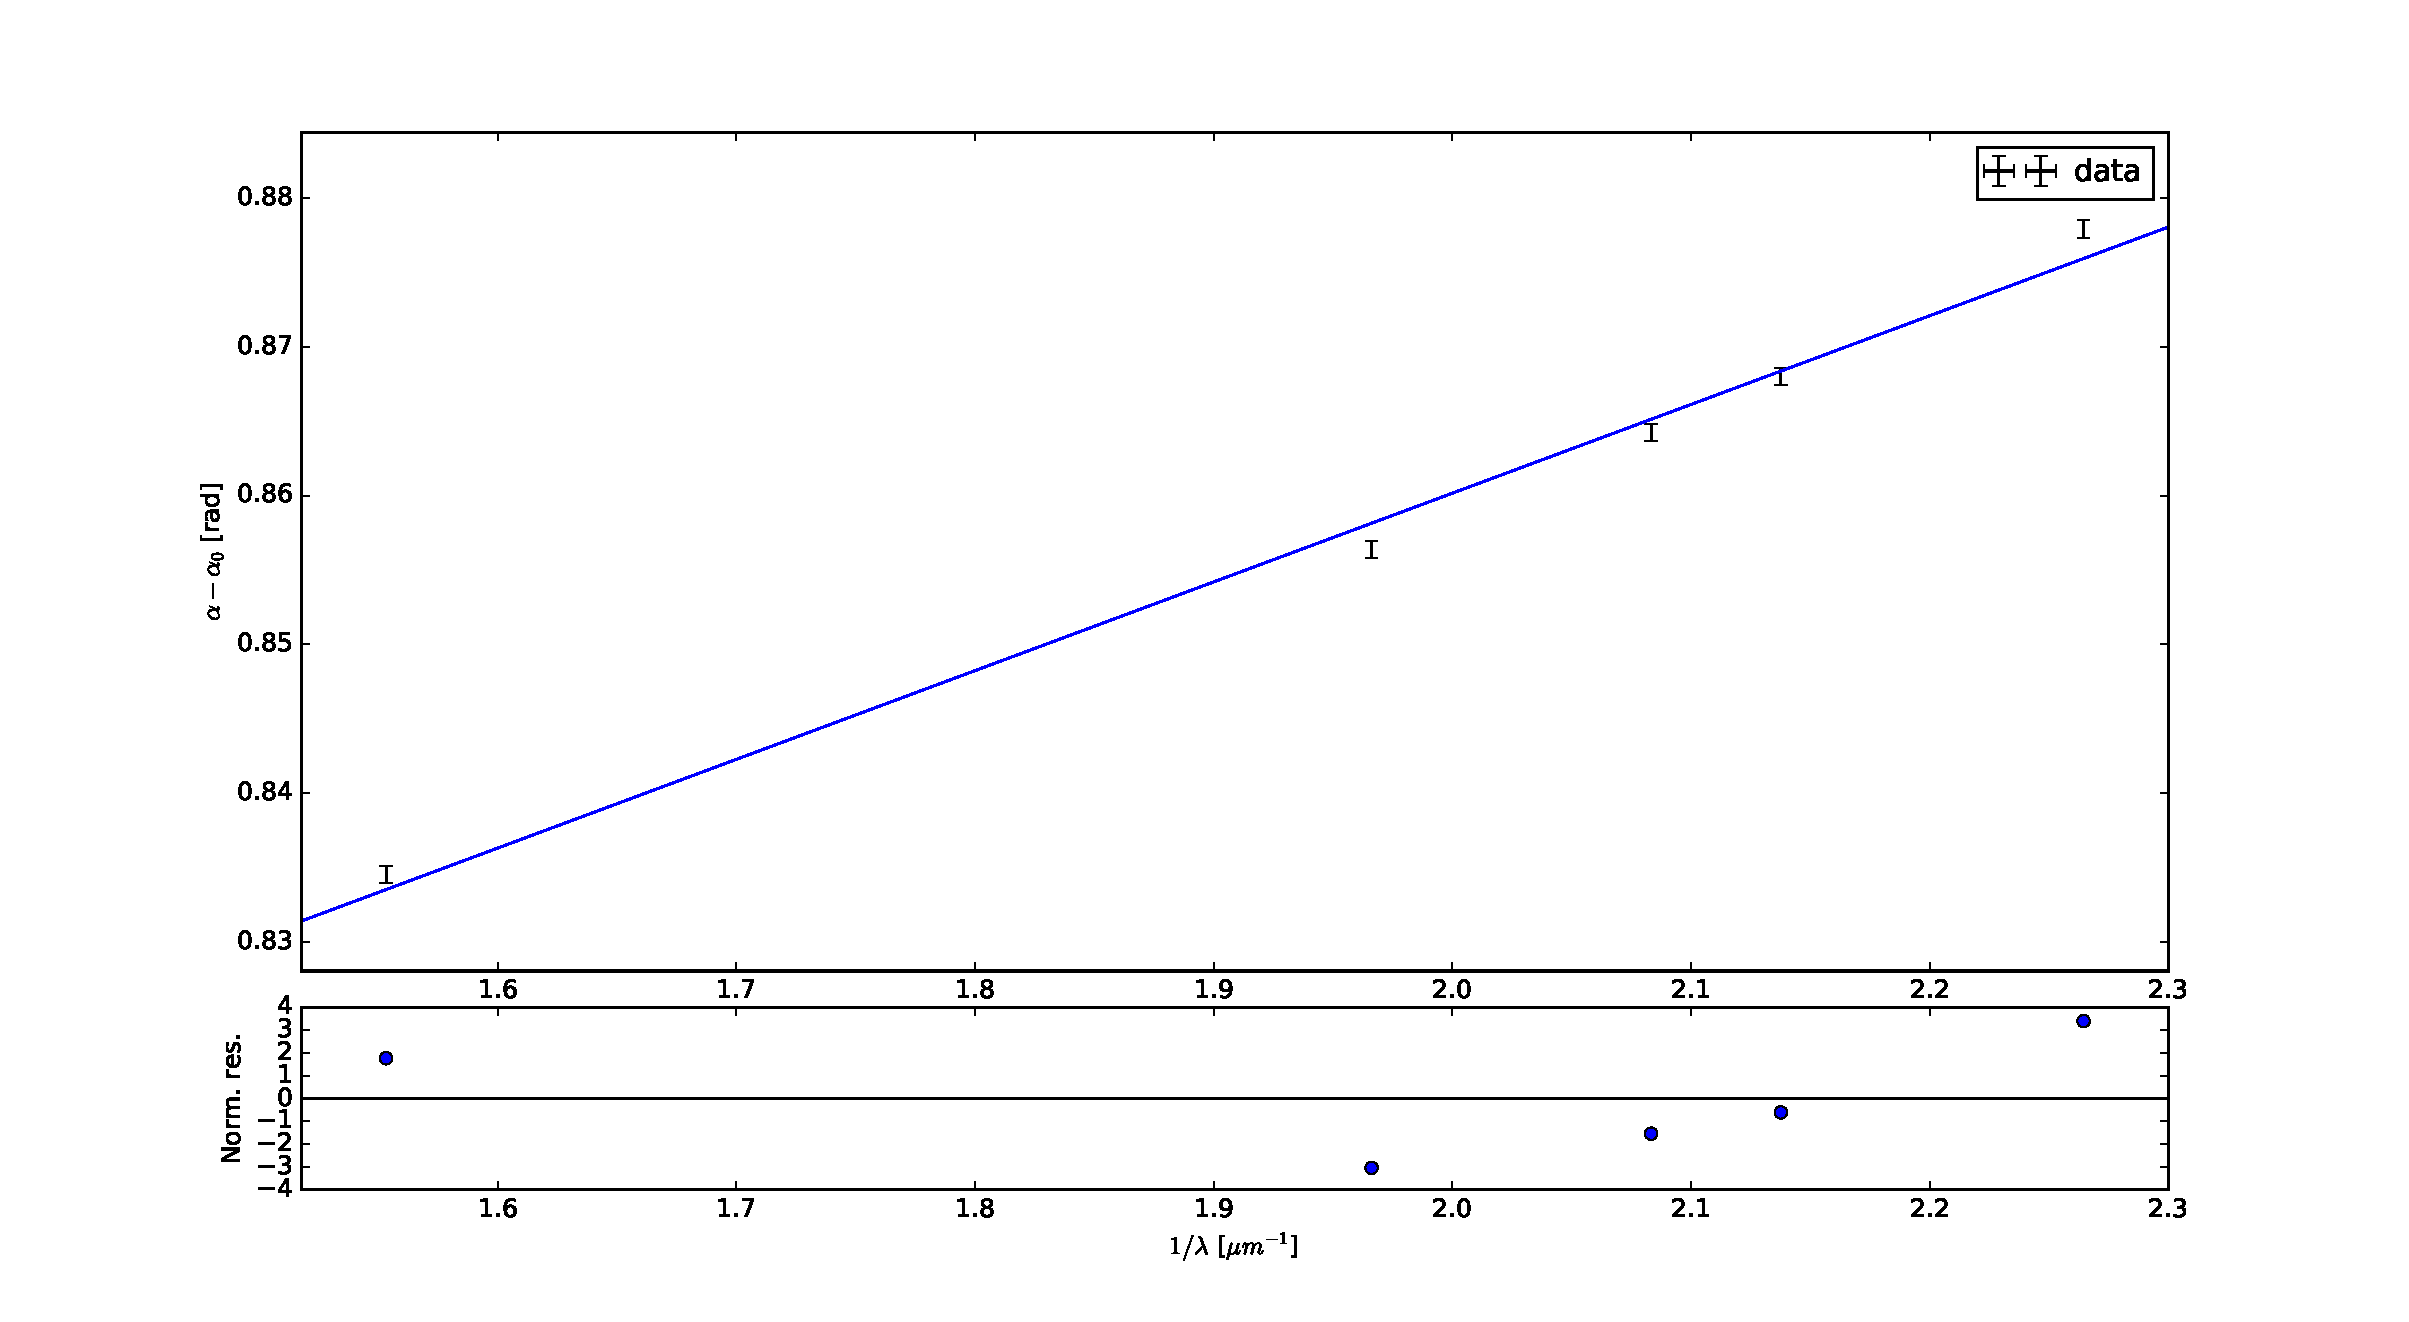
\includegraphics[scale=0.4]{fit_parteA.pdf}
		\caption{Posizione angolare contro $1/\lambda$ per le righe del cadmio e fit lineare.}
		\label{fig:fit_a}
	\end{figure}

	Il fit ha dato i seguenti valori: \\
	$m = \SI{0.0596 \pm 0.0011}{\radian\um}$ \\
	$q = \SI{0.7409 \pm 0.0022}{\radian}$ \\
	$\chi^2 = 11.8 \ (3 \dof , \  p = 0.0079) $ \\
	Con un coefficiente di correlazione di -0.992. L'alto $\chi^2$ è probabilmente
	dovuto al fatto che, a rigore, la condizione di minima deviazione vale solo
	per una delle righe spettrali misurate (quella verde), dunque non ci attendiamo
	che la relazione lineare sia esattamente verificata.

\subsection{Misura con lampada al sodio}
	Per effettuare le misure vere e proprie abbiamo
	rimontato la lampada al sodio in luogo di quella al cadmio.
	Dopo aver aspettato alcuni minuti, ritenuti necessari per la
	termalizzazione della sorgente, abbiamo osservato la posizione angolare
	$\alpha_{\text{Na}} = \angerr{48}{13(2)}$ della riga gialla del sodio.
	Dalla relazione tra quest'ultima e la lunghezza d'onda, utilizzando i parametri
	ottenuti attraverso il fit di calibrazione possiamo ricavare (tenuto conto
	anche della covarianza per la propagazione dell'errore):

	\begin{equation}
		\lambda_{\text{Na}} = \frac{m}{\alpha_{\text{Na}} - q} = \SI{592 (5)}{\nm}
	\end{equation}
	A fronte di un valore atteso di \SI{589}{\nm}, in ottimo accordo con quanto da noi misurato.
